%
% latex-sample.tex
%
% This LaTeX source file provides a template for a typical research paper.
%

%
% Use the standard article template.
%
\documentclass{article}

% The geometry package allows for easy page formatting.
\usepackage{geometry}
\geometry{letterpaper}

% Load up special logo commands.
\usepackage{doc}
\usepackage[utf8]{inputenc}
\usepackage[english]{babel}

\usepackage{amsthm}
 
\newtheorem*{remark}{Remark}
\newtheorem{example}{Example}

\usepackage{multirow}
\usepackage[table]{xcolor}

% itemize in table
\usepackage{booktabs}
\newcommand{\tabitem}{~~\llap{\textbullet}~~}
\usepackage{tabularx}
\usepackage{paralist}
\usepackage{pifont}
\usepackage{array}

% Package for formatting URLs.
\usepackage{url}

% Packages and definitions for graphics files.
\usepackage{graphicx}
\usepackage{epstopdf}
\usepackage{color}
\DeclareGraphicsRule{.tif}{png}{.png}{`convert #1 `dirname #1`/`basename #1 .tif`.png}

%
% Set the title, author, and date.
%
\title{DB2 Exam 610 Summary}
\author{Zeyuan Hu}
\date{\today}

% set indentation of paragraph
\setlength{\parindent}{0em}

%
% The document proper.
%
\begin{document}

% Add the title section.
\maketitle

% Add an abstract.
% \abstract{}

% Add various lists on new pages.
\pagebreak
\tableofcontents

% \pagebreak
% \listoffigures

% \pagebreak
% \listoftables

% Start the paper on a new page.
\pagebreak

%
% Body text.
%
\section{Planning}
\label{planning}

\subsection{Objectives}
\label{objectives}

\begin{itemize}
\item Knowledge of DB2 products (z/OS vs LUW vs pureScale - at a high-level; different products 
and what they do)
\item Knowledge of database workloads (appropriate DB2 product to use - OLTP vs warehousing)
\item Knowledge of non-relational data concepts (XML data, LOB data)
\end{itemize}

\subsection{Database workloads}
\label{database workloads}

Two main types of database application workloads:
\begin{itemize}
\item online transactional processing (OLTP)
\item data warehousing
\begin{itemize}
\item reporting
\item online analytical processing (OLAP)
\item data mining applications
\item decision support
\end{itemize}
\end{itemize}

\subsection{OLTP vs. Data Warehousing}
\label{oltp vs. data warehousing}

An OLTP system is typical of a web order system, where you perform transactions over the web
(such as ordering a product). Online transaction processing (OLTP) systems features:

\begin{itemize}
\item Support day-to-day, mission-critical business activities (ie. web-based order entry, stock trading)
[\textit{current data}]
\item Support hundreds to thousands of users issuing millions of transactions per day
against databases that vary in size [\textit{Frequent updates, Granular transactions}]
\item Response time requirements tend to be subsecond [\textit{Sub-second response time}]
\item Queries:
\begin{itemize}
\item tend to be a mix of real-time insert, update, and delete
operations against current-as opposed to historical-data
\item single-row lookups with logic that likely updates a small number of records
\end{itemize}
\end{itemize}


Data warehousing system typically consist of:
\begin{itemize}
\item Store and manage large volumes of data that is often historical in nature and is used primarily for
analysis [\textit{Voluminous historical data}]
\item Optimized for queries
\item Heterogeneous data sources
\item Queries: (ie. [\textit{Summarized queries that perform aggregations and joins}] )
\begin{itemize}
\item bulk load operations
\item short-running queries
\item long-running complex queries
\item random queries
\item occasional updates to data
\item execution of online utilities
\end{itemize}

\end{itemize}

\begin{example}
A database will be used primarily to identify sales patterns for products sold within the 
last three years and to summarize sales by region, on a quarterly basis. In case, a Data warehouse 
system is needed.
\end{example}

\begin{remark}
Different by {\color{red} queries that are typically used to access the data} (aka workloads).
\end{remark}


\begin{figure}[h]
\centering
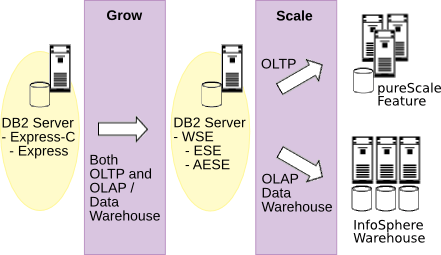
\includegraphics[scale=0.4]{workloads.png}
 
\caption{DB2 products, OLTP, Data Warehouse}
\label{workloads}
\end{figure}

\subsection{DB2 pureScale - IBM solution for OLTP}
\label{DB2 pureScale}

\medskip

System highlights:
\begin{itemize}
\item Best suited for OLTP workloads
\item Enables a \texttt{DB2 for LUW} database to continously process incoming requests, even if
multiple system components fail simultaneously, which makes it ideal for OLTP workloads where high
availability is crucial
\item Provides a database cluster solution for nonmainframe platforms
\item Can \textbf{ONLY} work with the General Parallel File System (GFPS) file system
\end{itemize}

\medskip

Usage:
\begin{itemize}
\item Can be used with \texttt{DB2 Workgroup Server Edition (WSE)}, \texttt{DB2 Enterprise Server Edition
(ESE)}, \texttt{DB2 Advanced Enterprise Server Edition(AESE)}
\item Can \textbf{ONLY} be installed on IBM p Series or x Series servers that are running either
the AIX (p Series) or the Linux (x Series) operating system
\item \textbf{CANNOT} be installed on IBM mainframes running z/OS, IBM p Series server running Linux,
or IBM x Series servers running Windows
\end{itemize}


\subsection{InfoSphere Warehouse - IBM solution for Data warehousing}

\medskip
System highlights:
\begin{itemize}
\item is a complete data warehousing solution that contains components that facilitate
data warehouse construction and administration, as well as tools that enable embedded data
mining and multidimensional online analytical processing (OLAP)
\end{itemize}

\subsection{Notable DB2 features \& products}

\textbf{IBM Data Studio}
\begin{itemize}
\item is an Eclipse-based, integrated development environment (IDE) that can be used to perform
instance and database administration, routine (SQL procedure, SQL functions, etc.) and application
development, and performance-tuning tasks.
\item replaces the \texttt{DB2 Control Center} as the standard GUI tool for DB2 database administration
and application development.
\item allows users to connect to a DB2 database using a wizard; however, users are required to provide
login credentials before a connection will be established.
\item components:
\begin{itemize}
\item \texttt{IBM Data Studio administration client}
\begin{itemize}
\item can be installed on servers running Red Hat Linux, SUSE Linux, and Windows
\item \textbf{CANNOT} be installed on AIX servers
\end{itemize}
\item \texttt{IBM Data Studio full client}
\begin{itemize}
\item can be installed on servers running Red Hat Linux, SUSE Linux, and Windows
\end{itemize}
\item \texttt{IBM Data Studio web console}
\begin{itemize}
\item can be installed on servers running Red Hat Linux, SUSE Linux, and Windows
\item can be installed on servers running the AIX operating system as well
\end{itemize}
\end{itemize}
\end{itemize}

\textbf{IBM Workload Manager (WLM)}
\begin{itemize}
\item is a comprehensive workload management feature that can help identify, manage, and control
database workloads to maximize database server throughput and resource utilization
\item cutomize execution environments for the purpose of  controlling system resources so that
no single workload can control and consume all of the system resources available. 
(This prevents any one department or service class from overwhelming the system.)
\end{itemize}

\textbf{IBM InfoSphere Optim Performance Manager Extended Edition}
\begin{itemize}
\item can be used to identify, diagnose, solve, and prevent performance problems in DB2 products and 
associated applications including Java and DB2 Call Level Interface (CLI) applications.
\end{itemize}

\textbf{Self-Tuning Memory Manager (STMM)}
\begin{itemize}
\item responds to significant changes in a database's workload by dynamically distributing available
memory resources among several different database memory consumers
\end{itemize}

\textbf{Connection Concentrator}
\begin{itemize}
\item improves the performance of applications that require frequent, but relatively transient, 
simultaneous user connections by allocating host database resources only for the duration of an 
SQL transaction,
\end{itemize}

\textbf{IBM InfoSphere Data Architect}
\begin{itemize}
\item A complete solution for designing, modeling, discovering, relating, and standardizing data assets.
\item You can use it for data modeling, transformation, and DDL generation, and to build, debug, and
manage database objects such as SQL stored procedures and functions.
\end{itemize}

\textbf{IBM InfoSphere Optim Query Tuner (Query Tuner)}
\begin{itemize}
\item can analyze and make recommendations on ways to tune existing queries, as well as provide expert
advice on writing new queries.
\end{itemize}

\textbf{IBM InfoSphere Optim pureQuery Runtime}
\begin{itemize}
\item Lets you deploy advanced pureQuery applications that use static SQL for a wide range of benefits.
\item Briges the gap between data and Java technology by harnessing the power of SQL within an easy-to-use
Java data access platform.
\item Increases security of Java applications helping to prevent threats like SQL injection.
\end{itemize}

\textbf{DB2 for i}
\begin{itemize}
\item combines with \texttt{IBM BLU Acceleration} to handle Analytical workloads
\item formerly known as DB2 for i5/OS, is an advanced, 64-bit Relational Database Management System
that leverages the high performance, virtualization, and energy efficiency features of IBM's Power Systems
\item its self-managing attributes, security, and built-in analytical processing functions make \texttt{
DB2 for i} an ideal database server for applications that are analytical in nature
\end{itemize}

\textbf{DB2 pureXML}
\begin{itemize}
\item offers a simple and efficient way to create a "hybrid" DB2 database that allows XML data
to be storded in its native, hierarchical format.
\end{itemize}

\textbf{Data Partitioning Feature (DPF)}
\begin{itemize}
\item provides the ability to divide very large databases into multiple parts (known as partitions) and
store them across a cluster of inexpensive servers.
\end{itemize}

\subsection{DB2 offering}
\textbf{DB2 for z/OS}
\begin{itemize}
\item full-function database management system that has been designed specifically for z/OS, IBM's
flagship mainframe operating system.
\item Tightly integrated with the IBM mainframe, \texttt{DB2 for z/OS} leverages the strengths of System
z 64-bit architecture to provide, among other things, the ability to support complex data warehouse.
\end{itemize}


\subsection{Large Objects (LOB)}

LOB data types-\textbf{not LOB locators}-are used to store binary data values in a DB2 database.
\begin{itemize}
\item By default, LOB data is stored in separate LOB storage objects.
\item Changes to LOB data are not recorded in transaction log files.
\end{itemize}

\smallskip

\textbf{Inline LOBs}
\begin{itemize}
\item improve query performance by storing LOB data in the same data pages as the rest of 
a table's rows, rather than in a separate LOB storage object.Thus, no additional I/O is needed to store and access this type of data. 
\item is eligible for compression.
\item When a table contains columns with inline LOBs, fewer rows can fit on a page.
\item transactions that modify inline LOB data are always logged. Consequently, the use of inline LOBs
can \textbf{increase} logging overhead.
\item are created by appending the \texttt{INLINE LENGTH} clause to a LOB column's definition.
\end{itemize}

\smallskip

\textbf{LOB locator}
\begin{itemize}
\item represents a value for a LOB resource that is stored in a database
\item is a simple token value that is used to refer to a much bigger LOB value
\item is a mechanism that refers to a LOB value from within a transaction
\item is \textbf{NOT} a data type, nor is it a database object
\item \textbf{do NOT} store copies of LOB data-they store a description of a base LOB value,
and the actual data that a LOB locator refers to is only materialized when it is assigned to a specific
location, such as an application host variable or another table record
\item they behave as a snapshot of a piece of an LOB value, and not as a pointer to a row or a location
in the database
\end{itemize}

\subsection{XML data}
\begin{itemize}
\item with \texttt{pureXML}, XML documents are stored in tables that contain one or more columns that have
been defined with the XML data type.
\item \texttt{CREATE TABLE employee (empid INT, resume XML)}
\end{itemize}

\newpage

\section{Security}
\label{security}

\subsection{Objectives}
\begin{itemize}
\item Knowledge of restricting data access
\item Knowledge of different privileges and authorities
\item Given a DCL SQL statement, knowledge to identify results (grant/revoke/connect statements)
\item Knowledge of Row and Column Access Control (RCAC)
\item Knowledge of Roles and Trusted Contexts
\end{itemize}

Three levels of security:
\begin{itemize}
\item level 1: control access to the instance under which a database was created
\item level 2: control access to the database itself
\item level 3: control access to the data and data objects reside within the database
\end{itemize}

\subsection{Authentication}
\begin{itemize}
\item is the process by which a system verifies a user's identity.
\item normally, an external facility (ie. OS, DCE) that is not pat of DB2 performs the authentication.
\item \textit{authentication type} for a server is a database manager configuration parameter to 
decide how and where users are authenticated.

\begin{center}
\begin{tabularx}{\textwidth}{l X}
\toprule
Type &  \multicolumn{1}{c}{Description}  \\ 
\midrule
\textbf{SERVER} & 
\begin{compactitem}[\ding{212}]
\item Authentication occurs on the server
\end{compactitem}
\\\hline
\textbf{SERVER\_ENCRYPT} &
\begin{compactitem}[\ding{212}]
\item Authentication occurs on the server
\item Passwords are encrypted at the client machine before being sent to the server
\end{compactitem}
\\\hline
\textbf{CLIENT} &
\begin{compactitem}[\ding{212}]
\item Authentication occurs at the client workstation, with no further checks on the server
\end{compactitem}
\\\hline
\textbf{KERBEROS} &
\begin{compactitem}[\ding{212}]
\item Authentication is performed by the Kerberos security software
\end{compactitem}  
\\\hline
\textbf{KRB\_SERVER\_ENCRYPT} &
\begin{compactitem}[\ding{212}]
\item Authentication is performed by Kerberos security software if the client's authentication 
type is set to KERBEROS. Otherwise, SERVER\_ENCRYPT is used
\end{compactitem} 
\\\hline
\textbf{DATA\_ENCRYPT} &
\begin{compactitem}[\ding{212}]
\item SERVER\_ENCRYPT
\item user data are encrypted
\end{compactitem}
\\\hline
\textbf{DATA\_ENCRYPT\_CMP} &
\begin{compactitem}[\ding{212}]
\item DATA\_ENCRYPT
\item Use SERVER\_ENCRYPT if DATA\_ENCRYPT not supported
\end{compactitem}
\\\hline
\textbf{GSSPLUGIN} &
\begin{compactitem}[\ding{212}]
\item Authentication is controlled by an external GSS-API plugin
\end{compactitem} 
\\\hline
\textbf{GSS\_SERVER\_ENCRYPT} &
\begin{compactitem}[\ding{212}]
\item GSSPLUGININ
\item Use SERVER\_ENCRYPT if GSSPLUGIN not supported
\end{compactitem}
\\
\bottomrule
\end{tabularx}
\end{center}


\end{itemize}


% \begin{table*}[h]
%    \begin{tabular}{l p{8cm}}
%        \hline \bfseries Name & \bfseries Opt 2 \\\hline 
%        \hline \bfseries Item 1 & \\\multicolumn{3}{|c|}{\parbox{0.9\textwidth}{
%            \begin{itemize}
%                \item Key 
%                \item Key 
%                \item Key 
%            \end{itemize} }}
%         \\ \bfseries Item 2 & X \\\multicolumn{3}{|c|}{\parbox{0.9\textwidth}{
%            \begin{itemize}
%                \item Key key key key key key key key key key key
%                \item Key key key key key key key key key key key
%                \item Key key key key key key
%            \end{itemize} }}
%         \\ \bfseries Item 3 &  & X\\\multicolumn{3}{|c|}{\parbox{0.9\textwidth}{
%            \begin{itemize}
%                \item Key
%             \end{itemize} }}
%          \\ \hline
%     \end{tabular}
%\end{table*}


% Generate the bibliography.
%\bibliography{latex-sample}
%\bibliographystyle{unsrt}

\end{document}
